%\documentclass[journal]{vgtc}                % final (journal style)
%\documentclass[review,journal]{vgtc}         % review (journal style)
%\documentclass[widereview]{vgtc}             % wide-spaced review
\documentclass[preprint,journal]{vgtc}       % preprint (journal style)
%\documentclass[electronic,journal]{vgtc}     % electronic version, journal

%% Uncomment one of the lines above depending on where your paper is
%% in the conference process. ``review'' and ``widereview'' are for review
%% submission, ``preprint'' is for pre-publication, and the final version
%% doesn't use a specific qualifier. Further, ``electronic'' includes
%% hyperreferences for more convenient online viewing.

%% Please use one of the ``review'' options in combination with the
%% assigned online id (see below) ONLY if your paper uses a double blind
%% review process. Some conferences, like IEEE Vis and InfoVis, have NOT
%% in the past.

%% Please note that the use of figures other than the optional teaser is not permitted on the first page
%% of the journal version.  Figures should begin on the second page and be
%% in CMYK or Grey scale format, otherwise, colour shifting may occur
%% during the printing process.  Papers submitted with figures other than the optional teaser on the
%% first page will be refused.

%% These three lines bring in essential packages: ``mathptmx'' for Type 1
%% typefaces, ``graphicx'' for inclusion of EPS figures. and ``times''
%% for proper handling of the times font family.

\usepackage{mathptmx}
\usepackage{graphicx}
\usepackage{times}
\usepackage{enumitem}
\usepackage{xspace}
\usepackage{array}
\usepackage{algorithm}
\usepackage{algpseudocode}
\usepackage{pifont}
\usepackage{paralist,array}
\usepackage{amsmath}

\makeatletter\let\MPtrue\@minipagetrue\makeatother
\newcommand{\ie}{\emph{i.e.,}\xspace}
\newcommand{\eg}{\emph{e.g.,}\xspace}
\newcommand{\etal}{\emph{et~al.}\xspace}

\usepackage{color}
%\usepackage[usenames,dvipsnames]{xcolor}
%\definecolor{Purple}{rgb}{.75,0,.85}
\newcommand{\remco}[1]{\textcolor{red}{(Remco: #1)}}


%% We encourage the use of mathptmx for consistent usage of times font
%% throughout the proceedings. However, if you encounter conflicts
%% with other math-related packages, you may want to disable it.

%% This turns references into clickable hyperlinks.
\usepackage[bookmarks,backref=true,linkcolor=black]{hyperref} %,colorlinks
\hypersetup{
  pdfauthor = {},
  pdftitle = {},
  pdfsubject = {},
  pdfkeywords = {},
  colorlinks=true,
  linkcolor= black,
  citecolor= black,
  pageanchor=true,
  urlcolor = black,
  plainpages = false,
  linktocpage
}

%% If you are submitting a paper to a conference for review with a double
%% blind reviewing process, please replace the value ``0'' below with your
%% OnlineID. Otherwise, you may safely leave it at ``0''.
\onlineid{0}

%% declare the category of your paper, only shown in review mode
\vgtccategory{Research}

%% allow for this line if you want the electronic option to work properly
\vgtcinsertpkg

%% In preprint mode you may define your own headline.
\preprinttext{6.830 Final project report, Fall 2015}

%% Paper title.

\title{Database Cracking: Concept Evaluation}

%% This is how authors are specified in the journal style

%% indicate IEEE Member or Student Member in form indicated below
\author{Zulsar Batmunkh\\
	\scriptsize MIT 
	\and Dana Mukusheva\\
	\scriptsize MIT 
	}
\authorfooter{
%% insert punctuation at end of each item
\item
Zulsar Batmunkh is MIT undergraduate. email: zulsar@mit.edu
\item
Dana Mukusheva is MIT undergraduate. email: mukushev@mit.edu
}

%other entries to be set up for journal
\shortauthortitle{Database Cracking: Concept Evaluation}
%\shortauthortitle{Firstauthor \MakeLowercase{\textit{et al.}}: Paper Title}

%% Abstract section.
\abstract{abstract goes here.}

%% Keywords that describe your work. Will show as 'Index Terms' in journal
%% please capitalize first letter and insert punctuation after last keyword
\keywords{}

%% ACM Computing Classification System (CCS). 
%% See <http://www.acm.org/class/1998/> for details.
%% The ``\CCScat'' command takes four arguments.

\CCScatlist{}

%% Uncomment below to disable the manuscript note
%\renewcommand{\manuscriptnotetxt}{}

%% Copyright space is enabled by default as required by guidelines.
%% It is disabled by the 'review' option or via the following command:
% \nocopyrightspace

%%%%%%%%%%%%%%%%%%%%%%%%%%%%%%%%%%%%%%%%%%%%%%%%%%%%%%%%%%%%%%%%
%%%%%%%%%%%%%%%%%%%%%% START OF THE PAPER %%%%%%%%%%%%%%%%%%%%%%
%%%%%%%%%%%%%%%%%%%%%%%%%%%%%%%%%%%%%%%%%%%%%%%%%%%%%%%%%%%%%%%%%

\begin{document}
\maketitle
%% The ``\maketitle'' command must be the first command after the
%% ``\begin{document}'' command. It prepares and prints the title block.

\section{Introduction}

Database cracking is the concept of partitioning and sorting the data on the fly based on the incoming query workload. While traditional index creation and maintenance requires upfront knowledge of query patterns and workloads, as well as costly human supervision, database cracking removes the need for human administration and efficiently manages database workload environments by treating index maintenance as a part of query processing. It continuously partitions the database into manageable pieces every time a new query is processed. Dynamic reorganization of data as the system is queried causes subsequent queries to run faster, irrespective of whether these queries had already been run.

In this paper, we analyze the relative performance of cracking in a simple single-column database that we have implemented for the purposes of this project. We conducted multiple experiments, with varying implementation details, workloads and query patterns. 

Section \ref{sec:background} presents the background on database cracking and related works. Section \ref{sec:system} includes the system overview and implementation details regarding our simplified database. We describe the details of our experiment setup in Section \ref{sec:experiments} and discuss the results of our findings and comparisons to already existing strategies in Section \ref{sec:discussion}. Finally, Section \ref{sec:conclusion} presents our conclusions.

\label{sec:introduction}

\section{Background}
\label{sec:background}
\subsection{Previous work}
Database cracking is an active research topic, which is led by a group of researchers from CWI Amsterdam. The concept of dynamic and query-considerate data partitioning was first introduced in \cite{kersten_2005}. It was then further developed into a cracking system with mature architecture and described in \cite{idreos_2007}. This system was built on top of MonetDB, a column-oriented database system. The authors also presented cracking algorithms that are used to partition the data, and conducted experiments and obtained evidence that cracking improves query execution performance in the long term. The performance was measured as cumulative time of query execution. In \cite{schuhknecht_2014}, the authors raised questions regarding the effects on the performance of cracking algorithm selection and cracker index implementation. Database cracking has many open questions and requires more experiments and research.

The previous work done in the field defined the experimental setup of our project. In particular, we have focused on column-store databases in order to qualitatively compare our results with ones obtained in \cite{idreos_2007}, which was also used as the source of the cracker algorithm. Moreover, we conducted experiments to analyze the performance of different cracker index implementations to prove the hypothesis stated in \cite{schuhknecht_2014}.

\subsection{Mechanism of Database Cracking}
The core idea of database cracking is to partition the column according to each incoming query, thereby, effectively reducing the size of partitions as more queries arrive. Such self-organizational behavior is desired when there is no upfront knowledge of query patterns, which would be required for preliminary creation of traditional indexes for the columns of interest. The database creates a copy of a column that was queried for the first time, which is referred to as the cracker column. Tuple relocation and swapping only happen in the cracker column, leaving the original column intact. Each subsequent query results in further data partitioning and spends less time on cracking the values, as the partition ranges become smaller and smaller.



\section{System Overview}
In  order to analyze the performance effects of the database cracking, we have implemented our own simple database system MiniDB. In this section we will describe components and implementation details of MiniDB.

MiniDB is a single column database implemented in Java, where each table consists of a single uniquely named column. The database keeps a mapping between a column name and a  column object in a hash map. The database table stores tuples as a list, and each tuple is a 32-bit integer. MiniDB maintains the following data structures: Simple Column, Sorted Column, Cracker Column, Cracker Index, Range Scan. 

\label{sec:system}

\subsection{MiniDB columns and indexes}


Simple Columns represent database tables and store tuples. They do not maintain a specific tuple order and insert a tuple to the end of the tuple list. In Simple Columns tuple lookup requires linear scan of the tuples list. 

Sorted Column is another data structure that represents database tables  which preserves the order of the tuples. Tuple lookup takes logarithmic time and is implemented as a binary search. 

Cracker Column is a data structure that cannot exist independently in the database, it can only be coupled with Simple Column that supports cracking, They are initialized and attached to a Simple Column instance after the first query. Cracker Columns contain same values as their corresponding Simple Columns, but in a different and constantly changing order. Cracker Columns store tuples in a partially sorted list, that is, once its tuples are reorganized and partitioned into two sublists (one with all tuples whose values are less than or equal to the partition value and one with all tuples whose values are greater than the partition value) Each Cracker Column is supplemented with a  Cracker Index instance. 

The Cracker Index instances are the data structures that are necessary to keep most-up-to date information about all partitions of the Cracker Column tuples. Particularly, Cracker Index stores pairs in the form $(v, p)$, where $v$ indicates that all tuples located at the positions less than and including $p$ have values less that and including $v$.

\subsection{Query processing}
MiniDB queries are the Range Scan objects that operate on a single column. Each Range Scan instance stores the pointer to its column of interest, endpoints of the value ranges, and the range sign, either one of $\leq$, $\textless$, $\geq$, $\textgreater$, $\textless \textless$, $\leq \textless$, $\textless \leq$, $\leq \leq$. Range Scan objects are essentially iterators on the values of their columns of interests. If the column does not support cracking, the iterator goes over all tuples and returns only those whose values belong to the specified range. Otherwise, they use cracking and simply iterate over all values that lie in a specified partition. 


\subsection{Cracker Index implementation}
Cracker Index functionality requires methods such as insert value-position pair, find predecessor of value $v$, find successor of value $v$ and lookup position $p$ of value $v$. Predecessor/successor search is used to define partitions with the closest boundaries, which is the case when a new unseen query arrives. We have implemented Cracker Index using three different underlying representations, AVL Tree, Sorted List and HashMap. Each of them has advantages and disadvantages in different scenarios.

\textbf{AVL Tree} stores value $v$ as a node key and a position $p$ as a node data. All of the operations on AVL Tree have logarithmic cost, which makes it a good candidates for large workloads. However, at the same time, the size of the tree grows with a number of queries, and maintaining the balance of the large tree might be costly.

\textbf{Hash Map} directly stores mapping between the value $v$ and the position $p$. The HashMap implementation is beneficial when all incoming queries are repetitive,and additional cracking is unnecessary, since the correct partition already exists. However, adding a new partition info into the index is costly, as predecessor/successor search takes linear time.

\textbf{Sorted List} stores value-position pairs a list sorted on values. Preserving the order of the list is costly and takes linear time, however, cheap successor and predecessor search balances the query cost.

\begin{table}
\begin{tabular}{| m{2em}  | m{2cm} | m{2cm}|  m{2cm} |} 
\hline
 & \textbf{AVL Tree}& \textbf{Hash Map}&\textbf{Sorted List} \\ 
\hline
\textbf{Pros} & Logarithmic insert, lookup, predecessor and successor search & Constant time lookup & Logarithmic lookup and constant predecessor and successor search \\
\hline
\textbf{Cons} & Cost for balance maintenance & Linear predecessor and successor search & Linear insert \\
\hline
\end{tabular}
\caption{Summary of cost-related advantages and disadvantages for each Cracker Index implementation.}
\label{table:implementations}
\end{table}

In Table \ref{table:implementations} we summarized pros and cons for each Cracker Index implementation.

\section{Experiments}
This section includes the detailed description of our experiments conducted to analyze the impact of database cracking on query execution performance. We use a similar setup for all performance evaluations. Our main focus is to study the impact of cracking the SELECT operator in memory. In order to identify relative performances, we ran same queries on the same column for all cracker index implementations and compared the results to two baselines: (1) simple scanning which scans the entire column and filters tuples satisfying the query and (2) sorting upfront 

\subsection{Experiment Setup}

\textbf{Hardware:} Amazon AWS server (8 GB memory) and MIT Athena computers (40 GB memory). 

\textbf{Dataset:} An array with one million distinct tuples of range 1 to 10${^6}$. 

\textbf{Workload:} Randomly generated 20000 queries with varying selectivity.

\textbf{Query ranges:} Open (single predicate), closed (lower and upper predicates) and mixed (randomly chosen to be either open or closed).
The predicates are chosen randomly from the range 1 to 10${^6}$.

\textbf{Selectivity:} 0.01 and 0.001. 

\textbf{Minimum Partition Size: } 100 and 1000.The cracker index could potentially become very large for non-repetitive queries and dividing columns further into small pieces would become highly costly. Therefore, we experimented with mentioned minimum partition sizes and not cracking the column any further.
\subsection{Performance of cracking index implementations}

\begin{figure}[h]
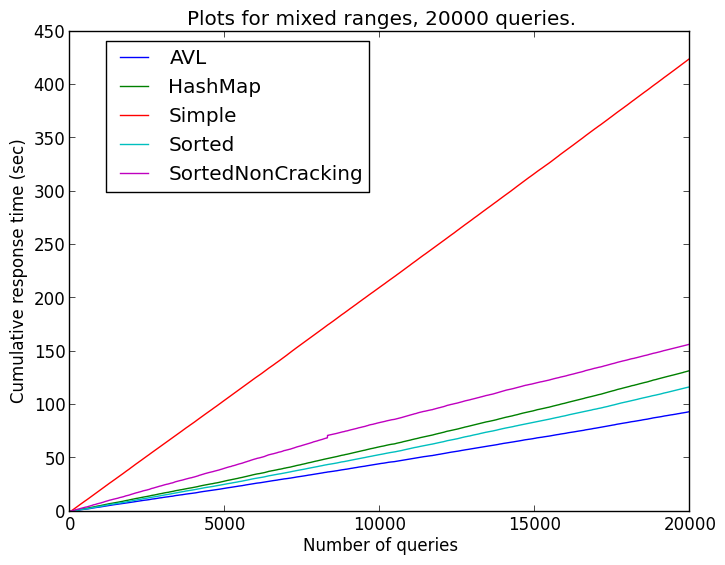
\includegraphics[width=8cm]{figures/mixed20000}
\caption{ADD CAPTION.}
\label{fig:some}
\end{figure}
include graph- -------

\subsubsection{Varying minimum partition size}


This approach simulates a sort based strategy. Upon a first query, the data column we sort the column upon the first query and operates upon the sorted column copy for the queries. This would potentially take O(logN) time for finding the correct start and/or end ranges for the query.

\subsubsection{Varying selectivity}

\textbf{Simple Scanning}
\label{sec:experiments}


\section{Discussion}
\indent The major concern regarding the results of our experiments and the conclusions we reached is the simplicity of our database-like environment. We have implemented our database to be a set of integer arrays; such implementation is missing many features and components of the existing commercial and research databases. For example, we have not used the notions of disk and cache, and our implementation is not cache-conscious.  Furthermore, our database is implemented in Java, which might not be the optimal choice for performance-sensitive systems. Additionally, MiniDB is limited to very primitive data structures and does not support more advanced and efficient algorithms. For example, \cite{schuhknecht_2014} mention more flexible and cost-efficient cracking algorithms, such as hybrid cracking, sideways cracking, and stochastic cracking.

Nevertheless, the concept of database cracking is efficient enough to show positive performance changes even in our simplified environment, thereby proving that it can potentially become an alternative to traditional database indexes. The database cracking idea was shown to be easily repeatable and extendable with varying parameters. The key advantages of the cracking approach are the self-adapting database based on the workload changes and the consequent elimination of human administration.
\label{sec:discussion}

\section{Conclusion}
Consistent with findings in previous works \cite{idreos_2007, schuhknecht_2014}, we found that as more and more queries arrive, the cost of physical data reorganization is amortized over all the queries, and the cracking approach outperforms both sorted-column scanning and traditional index (simple scanning) under changing workloads. In our simplified environment, we found each of the different cracker index implementations to have certain benefits and drawbacks with respect to each other, but all perform much faster than the baseline cumulative execution times. Even though our simple database lacks most of the key features of existing real-world databases, we still were able to verify that the cracking approach is indeed more efficient for queries of the form ``SELECT value  FROM column WHERE value  $\textless$ $x$". 

Overall, by using the cracker index the database automatically adapts to any workload and creates a re-organization that serves subsequent queries faster and faster. We believe that the database cracking idea has a great potential to revolutionize the traditional approach.
\label{sec:conclusion}




%\bibliography{ref}
%\bibliographystyle{abbrv}
\bibliographystyle{abbrv}
\bibliography{ref}{}

%\bibliographystyle{abbrv}
%\bibliography{paper}
\end{document}

